\documentclass{beamer}

%\colorlet{structure}{red!65!black}
%
%\beamertemplateshadingbackground{blue!40}{white}
%
\usepackage{beamerthemesplit}
%\usepackage{hyperref}
\usetheme{Berkeley}
\useinnertheme{circles}
\usecolortheme{seagull}

\title[Stereo vision]{Stereo Vision using the OpenCV library \\ Halfway report}
\author[Dr\"oppelmann \and Hueting \and Latour \and \\Van der Veen]{Sebastian Dr\"oppelmann \\ Moos Hueting \\ Sander Latour \\ Martijn van der Veen}
\institute{University of Amsterdam}
\date{June 2010}
\subject{Computer vision}

\begin{document}

\graphicspath{{./images/}}

\frame
{
  \titlepage
}

\section{Recap}

\frame
{
 \frametitle{Goal}
 \begin{block}{Goal}
   Generating a disparity depth map of the environment using stereo vision.
 \end{block}
}

\frame{
 \frametitle{Intended end-result}
 \begin{figure}
   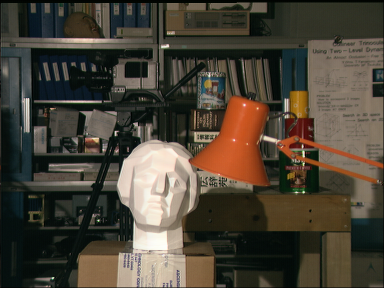
\includegraphics[width=0.3\textwidth]{exampleleft}
   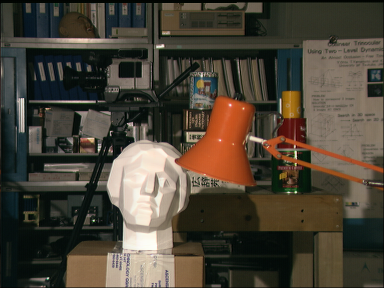
\includegraphics[width=0.3\textwidth]{exampleright}
   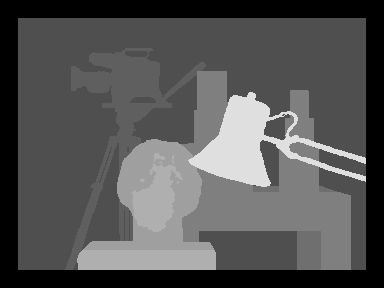
\includegraphics[width=0.3\textwidth]{exampledepth}
   \caption{Stereo images with disparity depth map}
 \end{figure}
}


\section{Results}

\frame{
 \frametitle{Stereo calibration}
 \begin{itemize}
   \item Estimating transformation between stereo camera pair
   \item Use chessboards
   \begin{itemize}
     \item Demo
   \end{itemize}
   \item Practical problems
\end{itemize}
}

\frame{
  \frametitle{Stereo rectification}
  \begin{itemize}
    \item Transform to make epipolar lines...
    \begin{itemize}
      \item ...horizontal
      \item ...colinear
    \end{itemize}
  \end{itemize}
}

\section{Planning}

\frame
{
  \frametitle{Tasks}
  \begin{itemize}
    \item Martijn and Moos
    \begin{itemize}
      \item Camera calibration
      \item Epipolar geometry
    \end{itemize}
    \item Sander and Sebastian
    \begin{itemize}
      \item Finding corresponding points
      \item Generating depth map
    \end{itemize}
  \end{itemize}
}

\frame
{
  \frametitle{Planning}
  \begin{itemize}
    \item Week 1
      \begin{itemize}
        \item Reading literature
        \item Getting webcams to work
        \item Choosing dense algorithm
      \end{itemize}
    \item Week 2 and 3
      \begin{itemize}
        \item Implementing
          \begin{itemize}
            \item Camera calibration
            \item Rectification of images using epipolar geometry
            \item Dense disparity map algorithm
          \end{itemize}
        \item Halfway report
      \end{itemize}
    \item Week 4
      \begin{itemize}
        \item Optimizing and testing
        \item If there's enough time left
          \begin{itemize}
            \item Generate 3D image of environment
            \item Remove background using dense disparity map
          \end{itemize}
      \end{itemize}
  \end{itemize}
}
\end{document}
